% =========================================================================
% CAPITOLO 9 — RISULTATI
% =========================================================================

\chapter{Risultati}
\label{ch:results}

\noindent
{\rmfamily\itshape
\begin{tabular}[t]{@{}l@{\hspace{0.3cm}}p{12.5cm}@{}}
\textls[50]{\textbf{Trattati:}} &
\textls[50]{Composizione del campione · Analisi descrittiva · Esiti della codifica · Comprensione
strutturale · Frequenza degli errori · Fiducia vs correttezza · Codici emergenti}
\end{tabular}
}

\vspace{0.5cm}

Questo capitolo riporta ciò che mostrano le risposte codificate: il campione, l'esito della codifica per ciascuna scena, la frequenza dell'errore sulla funzione di corrente, la relazione tra fiducia e correttezza, e la distribuzione dei codici emergenti tra le condizioni. La loro interpretazione, e la loro relazione con le aspettative del Capitolo~\ref{ch:userstudy}, è lasciata al Capitolo~\ref{ch:discussion}. Dato il campione di venticinque, tutte le cifre sono descrittive; i tre test esplorativi più sotto sono etichettati come tali e non sono trattati come inferenziali. Dimensioni dell'effetto e intervalli di confidenza non sono riportati: con dodici e tredici partecipanti per condizione i loro intervalli coprirebbero quasi tutto lo spazio dei parametri, e presentarli darebbe un'apparenza inferenziale a un confronto che questo capitolo non fa. L'artefatto la cui ricezione è qui riportata è documentato nel Capitolo~\ref{ch:translate}.\footnote{Tutti i conteggi e le tabelle di questo capitolo sono stati ricalcolati direttamente dall'insieme delle risposte codificate, conservato nel repository analitico documentato nella \S\ref{app:c-repos}.}

% -------------------------------------------------------------------------
\section{Composizione del campione}
\label{sec:res-sample}

Venticinque partecipanti hanno completato lo studio, dodici nella condizione di controllo e tredici nella sperimentale. La maggior parte aveva tra i 25 e i 34 anni (17 su 25). Il campione era molto istruito: quindici avevano una laurea magistrale, nove una triennale e uno un titolo di scuola secondaria superiore (Figura~\ref{fig:demographics}). Gli ambiti di studio e lavoro erano vari --- ingegneria, scienze, discipline umanistiche, sanità e arti --- senza alcun ambito rappresentato da più di due partecipanti.

La familiarità auto-valutata era bassa per il sistema specifico e moderata per le competenze correlate. La familiarità con l'AMOC era molto bassa (media 1,84 su una scala a dieci punti), quella con i temi climatici moderata (4,88), e quella con la lettura di visualizzazioni di dati la più alta delle tre (6,20).

Un controllo di equilibrio ha confrontato le due condizioni su queste misure (Figura~\ref{fig:balance}). Il gruppo sperimentale non era superiore a quello di controllo in nessuna di esse, ed era leggermente inferiore in tutte e tre; lo scarto maggiore era nella familiarità con le visualizzazioni di dati (5,54 contro 6,92 su una scala a dieci punti, una differenza di 1,38 punti).\footnote{Un confronto di Mann--Whitney colloca quello scarto a $p \approx 0.09$, riportato qui solo per completezza. L'entità e la direzione di uno squilibrio di partenza, non la sua significatività statistica, sono ciò che conta per l'interpretazione: un test di significatività sull'equilibrio di partenza risponde a una domanda che la randomizzazione ha già risolto.} La direzione conta: va nel verso che renderebbe più probabile l'errore della Scena~I nella condizione sperimentale (\S\ref{sec:res-misconception}), ed è ripresa nel Capitolo~\ref{ch:discussion}.


% -------------------------------------------------------------------------
\section{Comprensione strutturale per scena}
\label{sec:res-structure}

La quota di risposte codificate \emph{grasped} (colte) è variata nettamente tra le tre scene, e la direzione della differenza tra le condizioni non era la stessa in ciascuna (Figura~\ref{fig:grasped}).

Nella \textbf{Scena~I} (direzioni opposte con la profondità), le due condizioni erano vicine. Due terzi delle risposte di controllo (66,7\%) e una quota simile delle sperimentali (69,2\%) sono state codificate come grasped. Nella \textbf{Scena~II} (ricorrenza), nessun partecipante di controllo è stato codificato grasped (0 su 12), contro il 23,1\% nella condizione sperimentale (3 su 13); anche i codici \emph{partial} (parziale) sono aumentati nello stesso confronto, da due a cinque. Nella \textbf{Scena~III} (cambiamento nell'accordo tra modelli nel tempo), il pattern era invertito. Ogni partecipante di controllo è stato codificato grasped (12 su 12, 100\%), contro il 76,9\% nella condizione sperimentale (10 su 13).

Le risposte scritte mostrano ciò che i codici strutturali catturano. Nella Scena~I, una risposta grasped nominava direttamente l'inversione stratificata --- ``L'acqua non si muove in modo uniforme; vicino alla superficie e nella fascia medio-alta sembra più forte, e più in basso sembra invertirsi e tornare indietro nell'altra direzione'' (P11, controllo)\footnote{Originale (inglese), P11: ``The water doesn't move uniformly; near the top and the upper-middle it looks strongest, and lower down it seems to turn around and flow back the other way''.} --- mentre una parziale vedeva la variazione ma leggeva l'attraversamento dello zero come un arresto: ``c'è più acqua in movimento ad alcune profondità che ad altre, e le profondità intermedie sembrano averne di più \dots{} dove la linea tocca lo zero ho pensato che l'acqua si fermasse lì, e vicino al fondo sembrava andare nell'altra direzione, cosa che ho trovato strana'' (P08, controllo).\footnote{Originale (inglese), P08: ``there's more water moving at some depths than others, and the middle depths seem to have the most \dots{} where the line hits zero I assumed the water just stops there, and near the bottom it looked like it went the other way, which I found odd''.} Nella Scena~III, dove riconoscere l'accordo crescente bastava per essere codificati grasped, un partecipante di controllo ha scritto che nei primi anni i modelli ``non concordano molto'' ma ``concordano sempre di più nel tempo'' (P22, controllo);\footnote{Originale (inglese), P22: i modelli ``don't agree so much'' ma ``agree more and more over time''.} una risposta parziale ha invece trascinato la scena precedente, scambiando le tre rianalisi per i tre strati di profondità della Scena~I: ``vanno abbastanza di pari passo, soprattutto il secondo e terzo modello, immagino siano i tre strati con direzioni che cambiano'' (P01, sperimentale).

Un test esatto di Fisher è stato condotto una volta per scena, sulla tabella due-per-due di grasped contro not-grasped. Ha restituito $p = 1.00$ per la Scena~I, $p = 0.22$ per la Scena~II e $p = 0.22$ per la Scena~III. Tutti e tre sono esplorativi.\footnote{Solo tre test, uno per scena, fissati in anticipo. Not-grasped accorpa \emph{partial} e \emph{not\_grasped}. Nessun test è corretto per confronti multipli o letto come inferenziale, in linea con la dimensione campionaria indicata nel Capitolo~\ref{ch:userstudy}.} La Tabella~\ref{tab:grasped-counts} riporta i conteggi sottostanti.

\begin{table}[tbp]
\centering
\caption[Esiti della codifica strutturale per condizione e scena]{Conteggi di \emph{grasped} (colto), \emph{partial} (parziale) e \emph{not grasped} (non colto) per condizione e scena. Le percentuali nel testo sono sul totale della condizione (controllo $n=12$, sperimentale $n=13$).}
\label{tab:grasped-counts}
\small
\renewcommand{\arraystretch}{1.3}
\begin{tabularx}{\textwidth}{@{}l l *{3}{>{\centering\arraybackslash}X} @{}}
\toprule
\textbf{Scena} & \textbf{Condizione} & \textbf{Grasped} & \textbf{Partial} & \textbf{Not grasped} \\
\midrule
I   & Controllo    & 8 & 3 & 1 \\
I   & Sperimentale & 9 & 2 & 2 \\
\midrule
II  & Controllo    & 0 & 2 & 10 \\
II  & Sperimentale & 3 & 5 & 5 \\
\midrule
III & Controllo    & 12 & 0 & 0 \\
III & Sperimentale & 10 & 3 & 0 \\
\bottomrule
\end{tabularx}
\end{table}

% -------------------------------------------------------------------------
\section{L'errore sulla funzione di corrente}
\label{sec:res-misconception}

Un codice diagnostico, S1-MISC-INT, registrava se un partecipante leggesse l'altezza della curva della funzione di corrente come la velocità dell'acqua a quella profondità, anziché come il trasporto cumulato. Era presente in 14 delle 25 risposte alla Scena~I. Un partecipante ha enunciato la sostituzione chiaramente: ``Ho dato per scontato che l'acqua più veloce significasse che si muoveva più acqua, ma non sono sicuro che sia giusto'' (P20, sperimentale),\footnote{Originale (inglese), P20: ``I assumed the fastest water meant the most water was being moved, but I'm not certain that's right''.} leggendo la velocità delle particelle in movimento come la quantità d'acqua trasportata.

La sua frequenza differiva per condizione: 33,3\% delle risposte di controllo contro 76,9\% delle sperimentali. Suddiviso invece per familiarità auto-valutata con le visualizzazioni di dati, era presente nel 76,9\% dei partecipanti pari o al di sotto del punto mediano del campione e nel 33,3\% di quelli al di sopra (Figura~\ref{fig:misconception}).

Il codice era indipendente dal fatto che la scena fosse grasped: diversi partecipanti che hanno descritto correttamente le direzioni opposte leggevano comunque l'altezza della curva come velocità, portando sia il verdetto grasped sia l'errore.\footnote{Poiché la condizione sperimentale aveva anche una familiarità media più bassa con le visualizzazioni di dati (\S\ref{sec:res-sample}), condizione e familiarità sono in parte confuse a questa dimensione campionaria. Si noti che le due suddivisioni producono gli stessi conteggi (dieci su tredici contro quattro su dodici in entrambe), il che indica che sono vicine alla stessa partizione del campione anziché due viste indipendenti di essa. I due pannelli della Figura~\ref{fig:misconception} vanno quindi letti come un'unica osservazione confusa, e la loro lettura congiunta è esplorativa. Questo punto è ripreso nel Capitolo~\ref{ch:discussion}.} Tre partecipanti hanno distinto esplicitamente il trasporto cumulato dalla velocità e non portavano il codice; due di loro hanno anche chiesto, spontaneamente, che l'asse fosse etichettato per mostrare quale quantità rappresentasse.

% -------------------------------------------------------------------------
\section{Fiducia e correttezza}
\label{sec:res-confidence}

La fiducia media era più alta per le risposte grasped che per quelle non grasped in ogni scena, ma lo scarto variava (Figura~\ref{fig:confidence}): più ampio nella Scena~II (6,33 contro 4,27) e nella Scena~III (6,32 contro 4,67), più stretto nella Scena~I (6,82 contro 6,0 sulle otto non grasped). Gli scarti delle Scene~II e~III poggiano ciascuno su un sottogruppo di tre e vanno letti di conseguenza.

La definizione fissata a priori di risposta sicura-ma-errata era una fiducia di almeno sette insieme a un verdetto \emph{not\_grasped}. Sotto questa definizione, nessun caso simile è comparso nella Scena~I. Una lettura più ampia, che ammette anche verdetti \emph{partial}, ha individuato quattro partecipanti della Scena~I (P02, P04, P12 e P17) che hanno valutato la propria fiducia a sette o più pur essendo codificati solo partial. Ciascuno di questi quattro portava l'errore sulla funzione di corrente.\footnote{Questa lettura più ampia è riportata come osservazione post-hoc ed è tenuta separata dalla definizione fissata a priori, che non restituisce casi nella Scena~I. I quattro partecipanti sono segnati nella Figura~\ref{fig:confidence}.} Altri due casi compaiono nella Scena~II sotto la stessa lettura più ampia, uno per condizione, e nessuno nella Scena~III.

% -------------------------------------------------------------------------
\section{Codici emergenti}
\label{sec:res-emergent}

La codifica ha fatto emergere anche pattern al di fuori della griglia definita a priori, riportati come post-hoc e tenuti separati dai target strutturali.\footnote{L'elenco completo dei codici emergenti, inclusi quelli occorsi una sola volta, è dato nell'Appendice~\ref{app:protocols}; la Figura~\ref{fig:emergent-full} li mostra tutti per condizione. Qui sono descritti solo i tre codici ricorrenti.} Tre sono occorsi abbastanza spesso da essere riportati per condizione (Figura~\ref{fig:emergent}). \textsc{Interaction-aided}, che segna una risposta che attribuiva la propria comprensione all'agire sul display (mettere in pausa, riavvolgere, isolare), è comparso 12 volte, tutte nella condizione sperimentale. \textsc{Static-limit-named}, che segna una risposta che nominava l'assenza di un ordinamento temporale come la ragione per cui non poteva dire se il sistema ripassasse per stati precedenti, è comparso 4 volte, tutte nella condizione di controllo. \textsc{Anomaly-confusion}, che segna la difficoltà con la codifica usuale/insolito, è comparso 6 volte, una nella condizione di controllo e cinque nella sperimentale.

Con le parole dei partecipanti, le due condizioni descrivono lo stesso confine da lati opposti. Un partecipante sperimentale ha attribuito la lettura al seguire il movimento: ``Seguendo la traiettoria nel tempo è chiaramente irregolare, ma non priva di memoria --- ripassa per intorni di stati precedenti anziché allontanarsi, perciò il sistema sembra poter tornare a configurazioni passate'' (P18, sperimentale).\footnote{Originale (inglese), P18: ``Following the trajectory over time it's clearly irregular, but not memoryless --- it revisits neighbourhoods of earlier states rather than wandering off, so the system looks like it can return to previous configurations''.} Un partecipante di controllo ha nominato esattamente ciò che lo scatter immobile tratteneva: ``Difficile dirlo da un'immagine statica. I punti sembrano sparpagliati attorno a una zona centrale, il che fa pensare a un moto irregolare, ma senza un ordine temporale non riesco a stabilire se il sistema ripassi per stati simili'' (P24, controllo).

Due ulteriori misure raccolte sono riportate qui solo brevemente. Il codice \textsc{Uncertainty-as-quality} --- incertezza produttiva, in cui un partecipante nominava ciò che un display non gli diceva anziché tirare a indovinare --- è stato applicato a ogni risposta ed era presente in 41 delle 75, in entrambe le condizioni; è registrato come segnale positivo che i formati invitavano a un'onesta cautela anziché come confronto tra condizioni. I tre item di riflessione conclusivi (Q19--Q21: comprensione complessiva, ciò che è rimasto poco chiaro, e se l'esperienza abbia cambiato la visione del sistema del partecipante) sono stati raccolti per contesto e per guidare un'iterazione futura; informano la discussione nel Capitolo~\ref{ch:discussion} anziché i risultati codificati qui riportati.

% -------------------------------------------------------------------------
% FIGURE
% -------------------------------------------------------------------------

\begin{figure}[tbp]
\centering
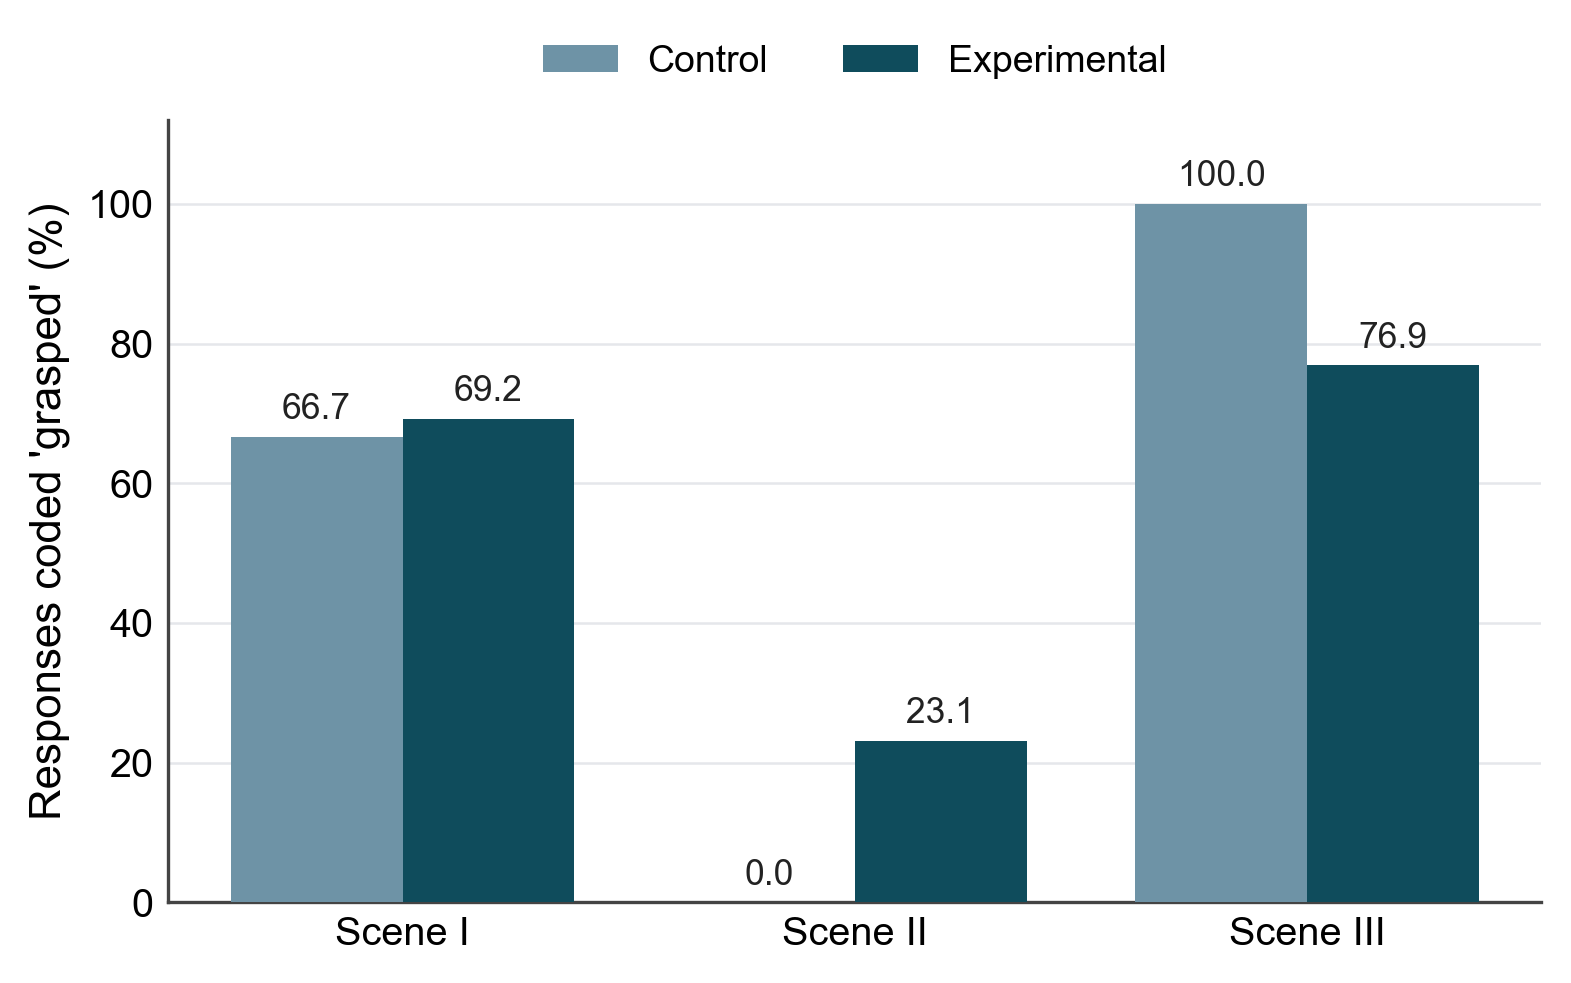
\includegraphics[width=\textwidth]{figures/results/F1_grasped_by_condition_scene.png}
\caption[Comprensione strutturale per condizione e scena]{Percentuale di risposte codificate \emph{grasped} per condizione, per ciascuna scena. La direzione della differenza tra le due condizioni non è la stessa nelle tre scene.}
\label{fig:grasped}
\end{figure}

\begin{figure}[tbp]
\centering
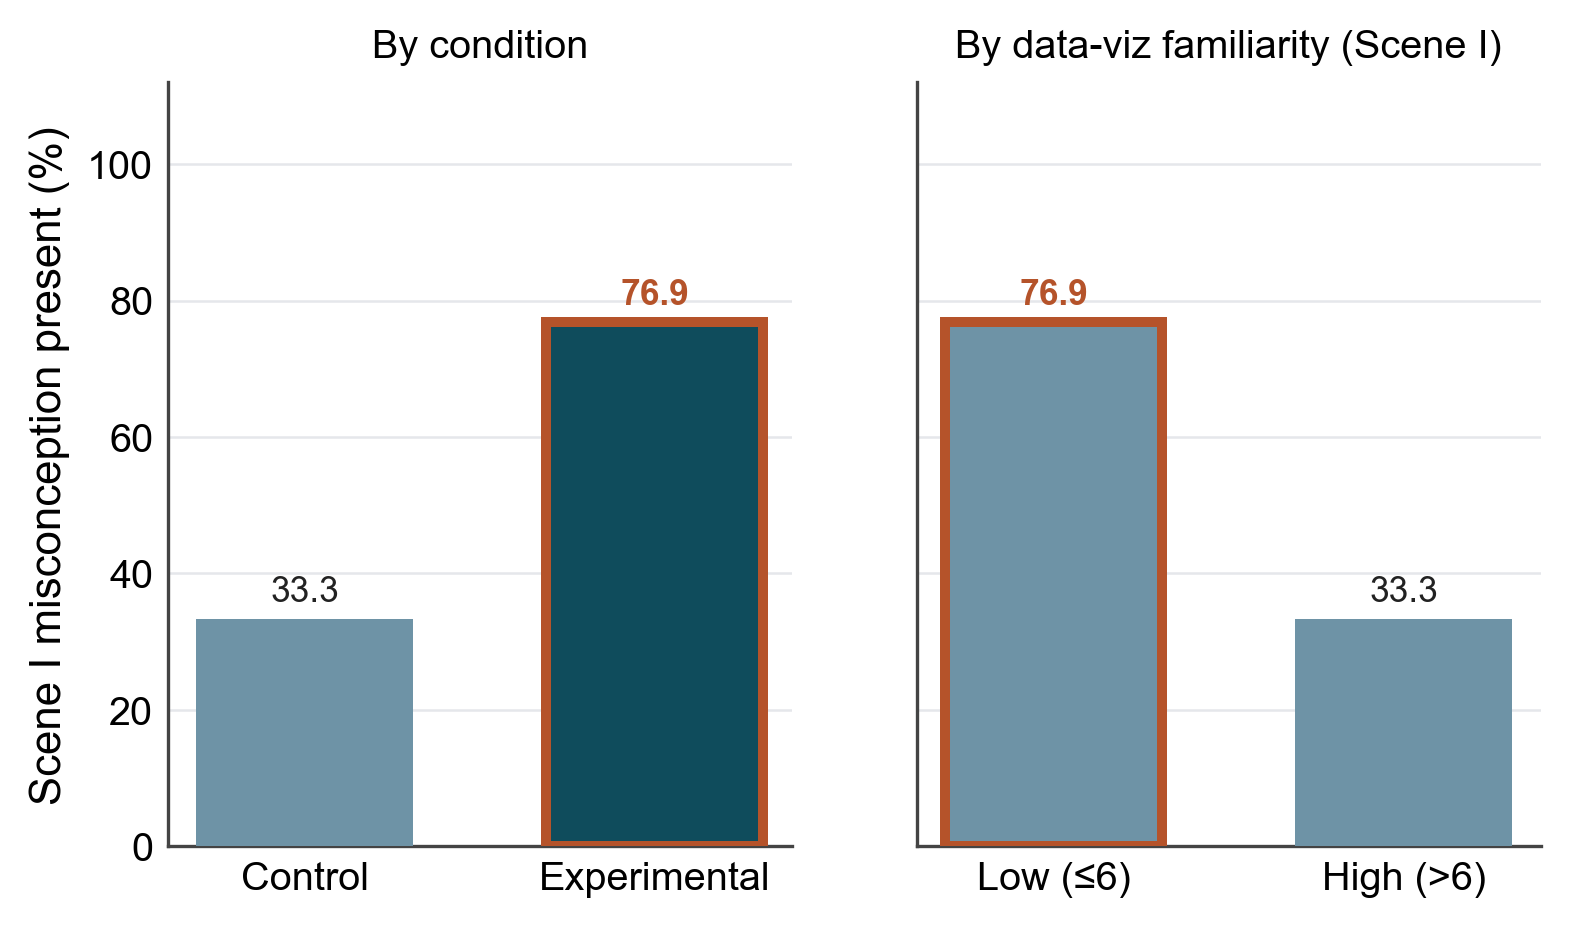
\includegraphics[width=\textwidth]{figures/results/F2_misconception.png}
\caption[L'errore sulla funzione di corrente, per condizione e per familiarità]{Presenza dell'errore S1-MISC-INT nella Scena~I. A sinistra: per condizione. A destra: per familiarità auto-valutata con le visualizzazioni di dati. I due pannelli sono in parte confusi (vedi \S\ref{sec:res-misconception}).}
\label{fig:misconception}
\end{figure}

\begin{figure}[tbp]
\centering
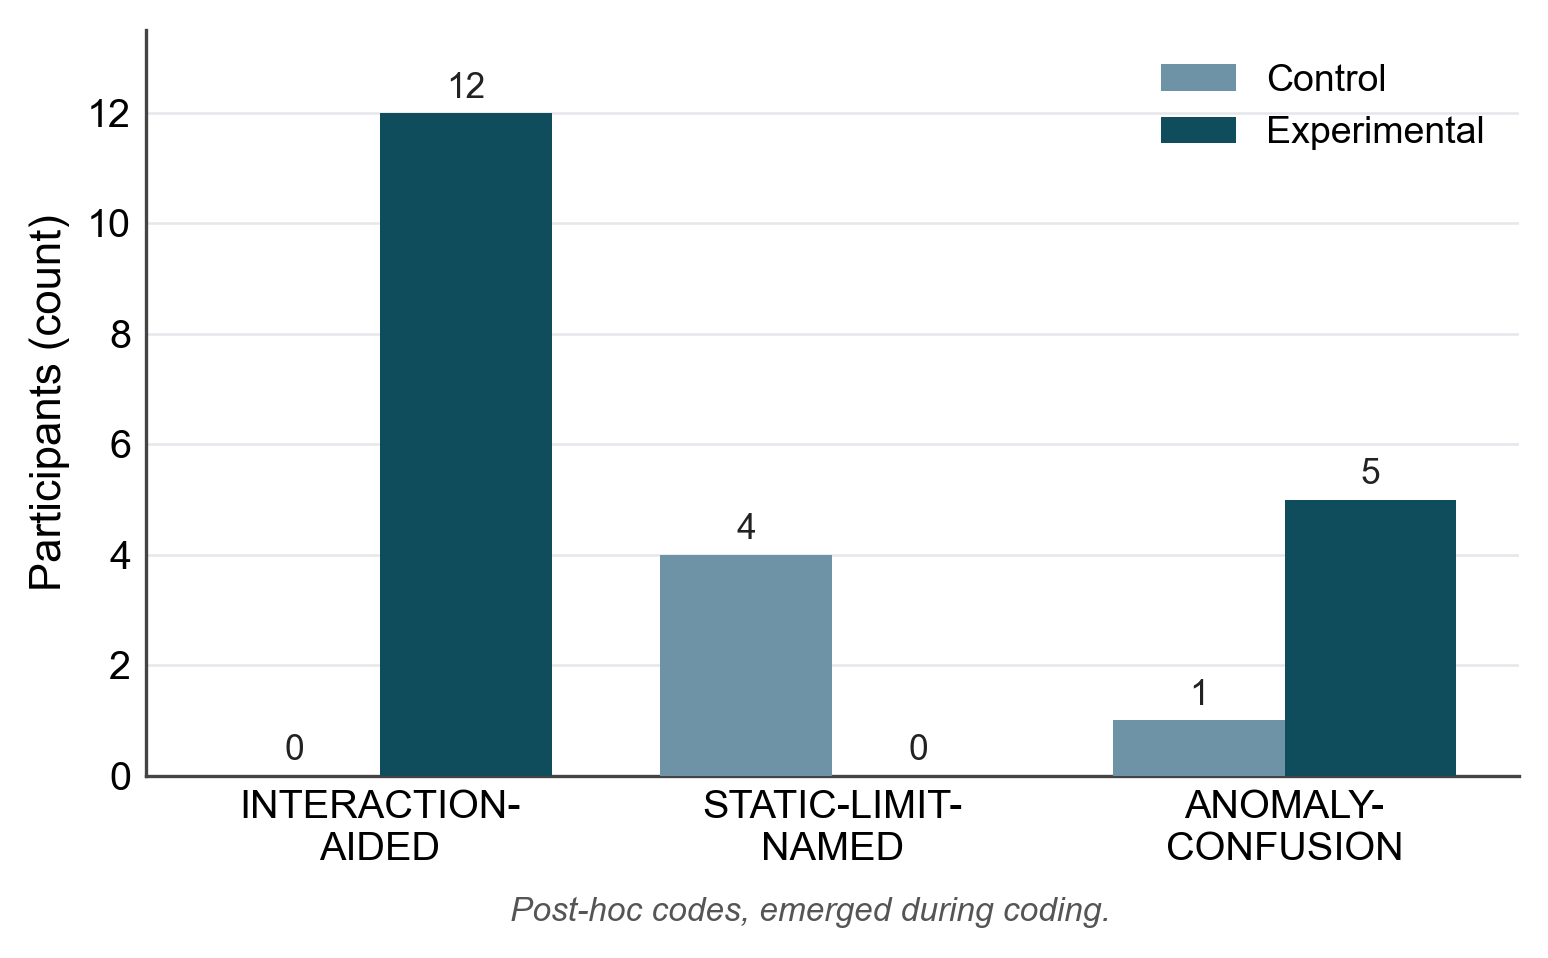
\includegraphics[width=\textwidth]{figures/results/F3_emergent_mechanism.png}
\caption[Codici emergenti ricorrenti per condizione]{I tre codici emergenti ricorrenti per condizione. I primi due sono immagini speculari l'uno dell'altro; il terzo va contro la condizione sperimentale. Codici post-hoc emersi durante la codifica; non parte della griglia definita a priori.}
\label{fig:emergent}
\end{figure}

\begin{figure}[tbp]
\centering
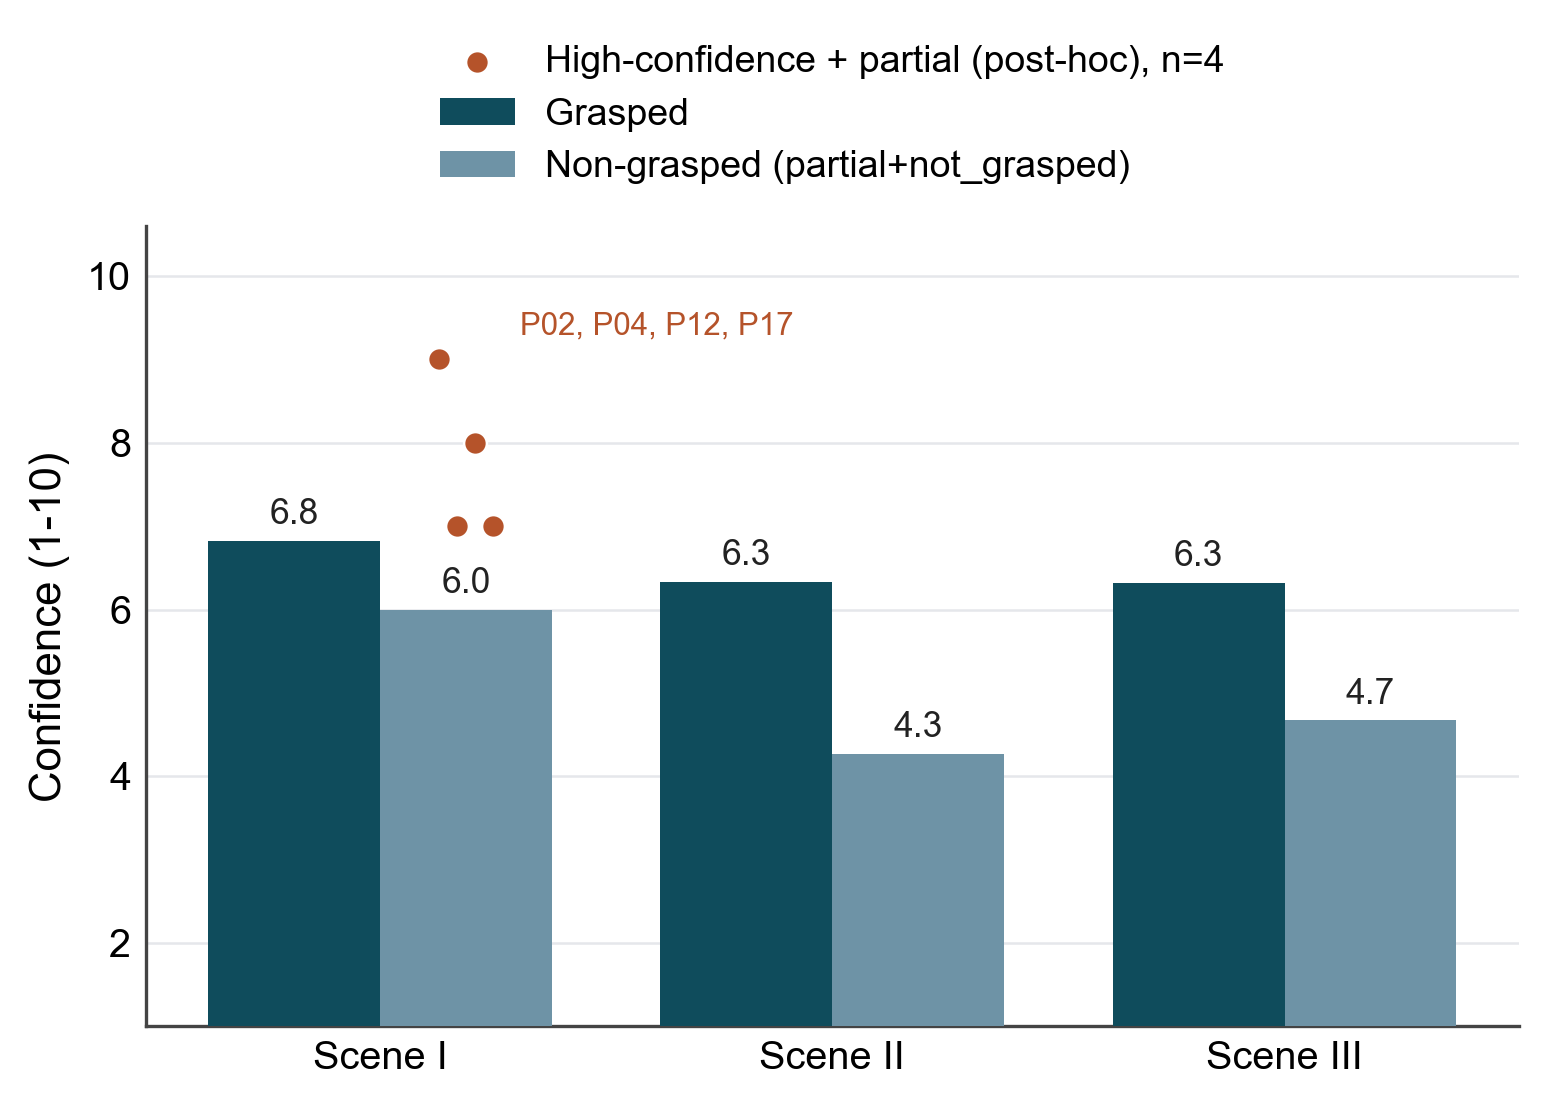
\includegraphics[width=\textwidth]{figures/results/F4_confidence_by_correctness.png}
\caption[Fiducia per correttezza e scena]{Fiducia media delle risposte grasped contro non grasped (partial e not-grasped accorpate), per scena. I quattro punti evidenziati segnano i partecipanti della Scena~I con fiducia $\geq 7$ e verdetto partial (lettura post-hoc; vedi \S\ref{sec:res-confidence}).}
\label{fig:confidence}
\end{figure}

\begin{figure}[tbp]
\centering
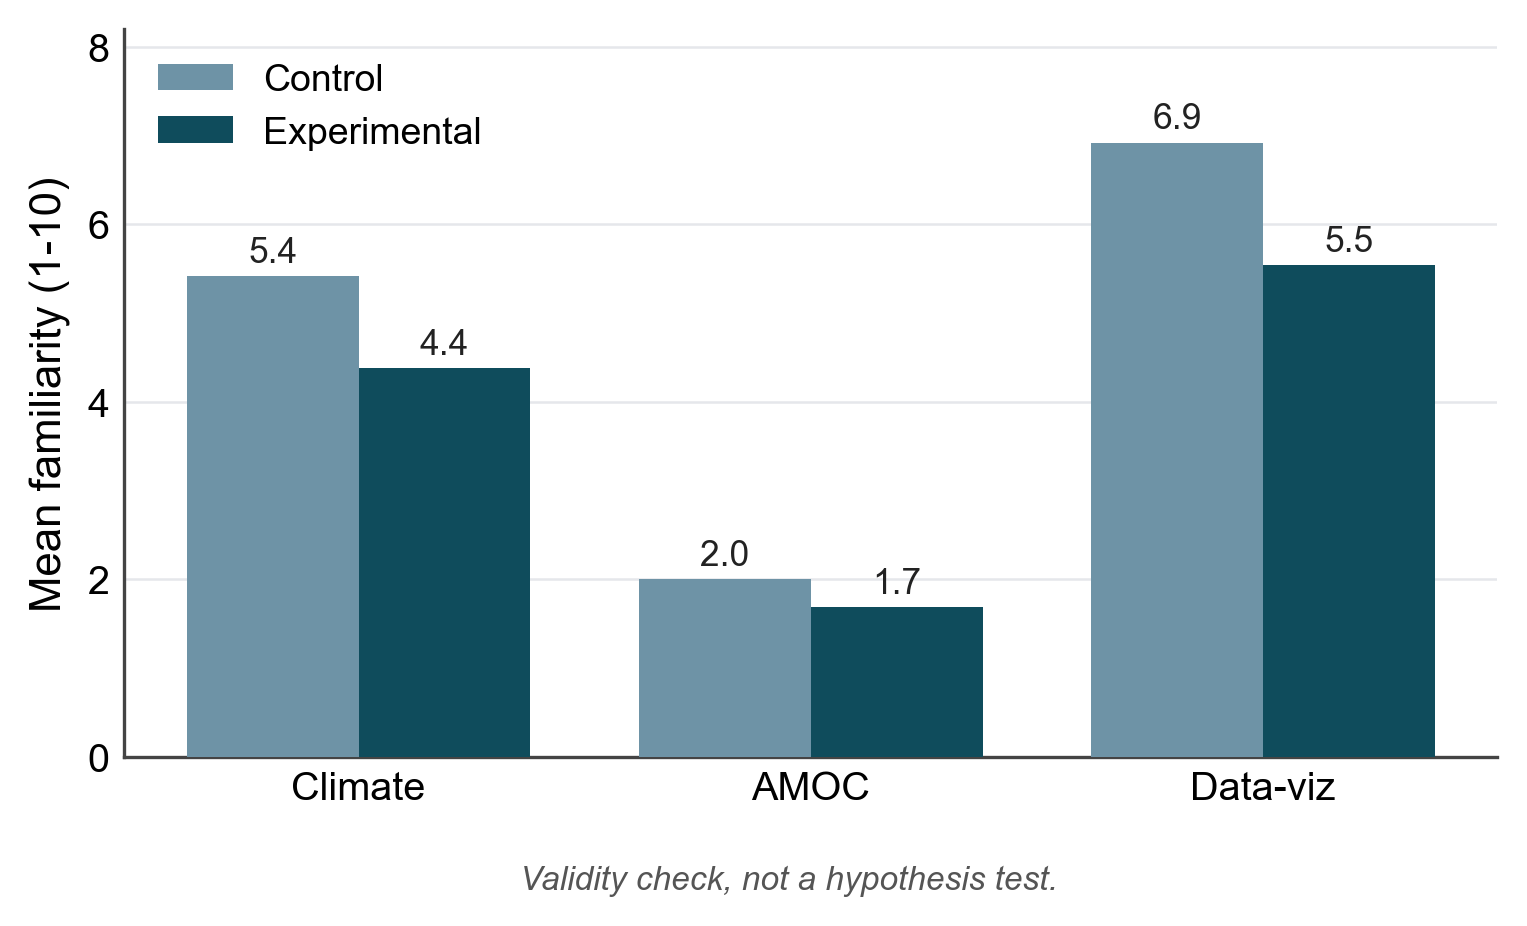
\includegraphics[width=\textwidth]{figures/results/S1_balance_familiarity.png}
\caption[Controllo di equilibrio: familiarità per condizione]{Familiarità media auto-valutata sulle tre misure, per condizione. Un controllo di equivalenza tra gruppi, non un test di ipotesi.}
\label{fig:balance}
\end{figure}

\begin{figure}[tbp]
\centering
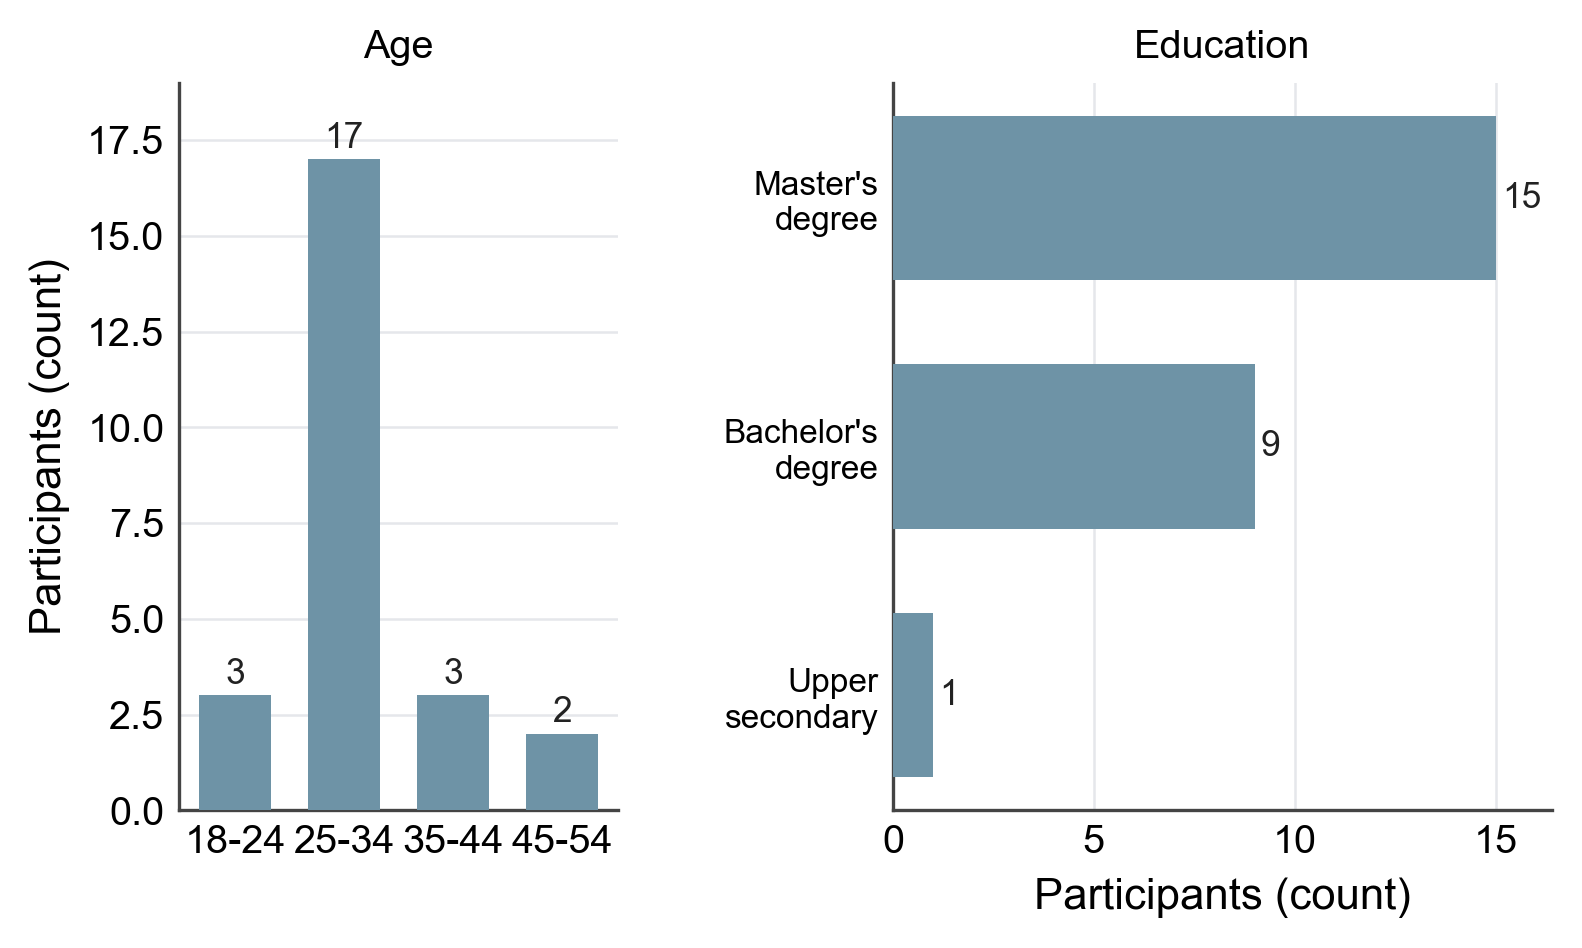
\includegraphics[width=\textwidth]{figures/results/S2_demographics.png}
\caption[Dati demografici del campione]{Distribuzione della fascia d'età e del titolo di studio più elevato nel campione.}
\label{fig:demographics}
\end{figure}

\begin{figure}[tbp]
\centering
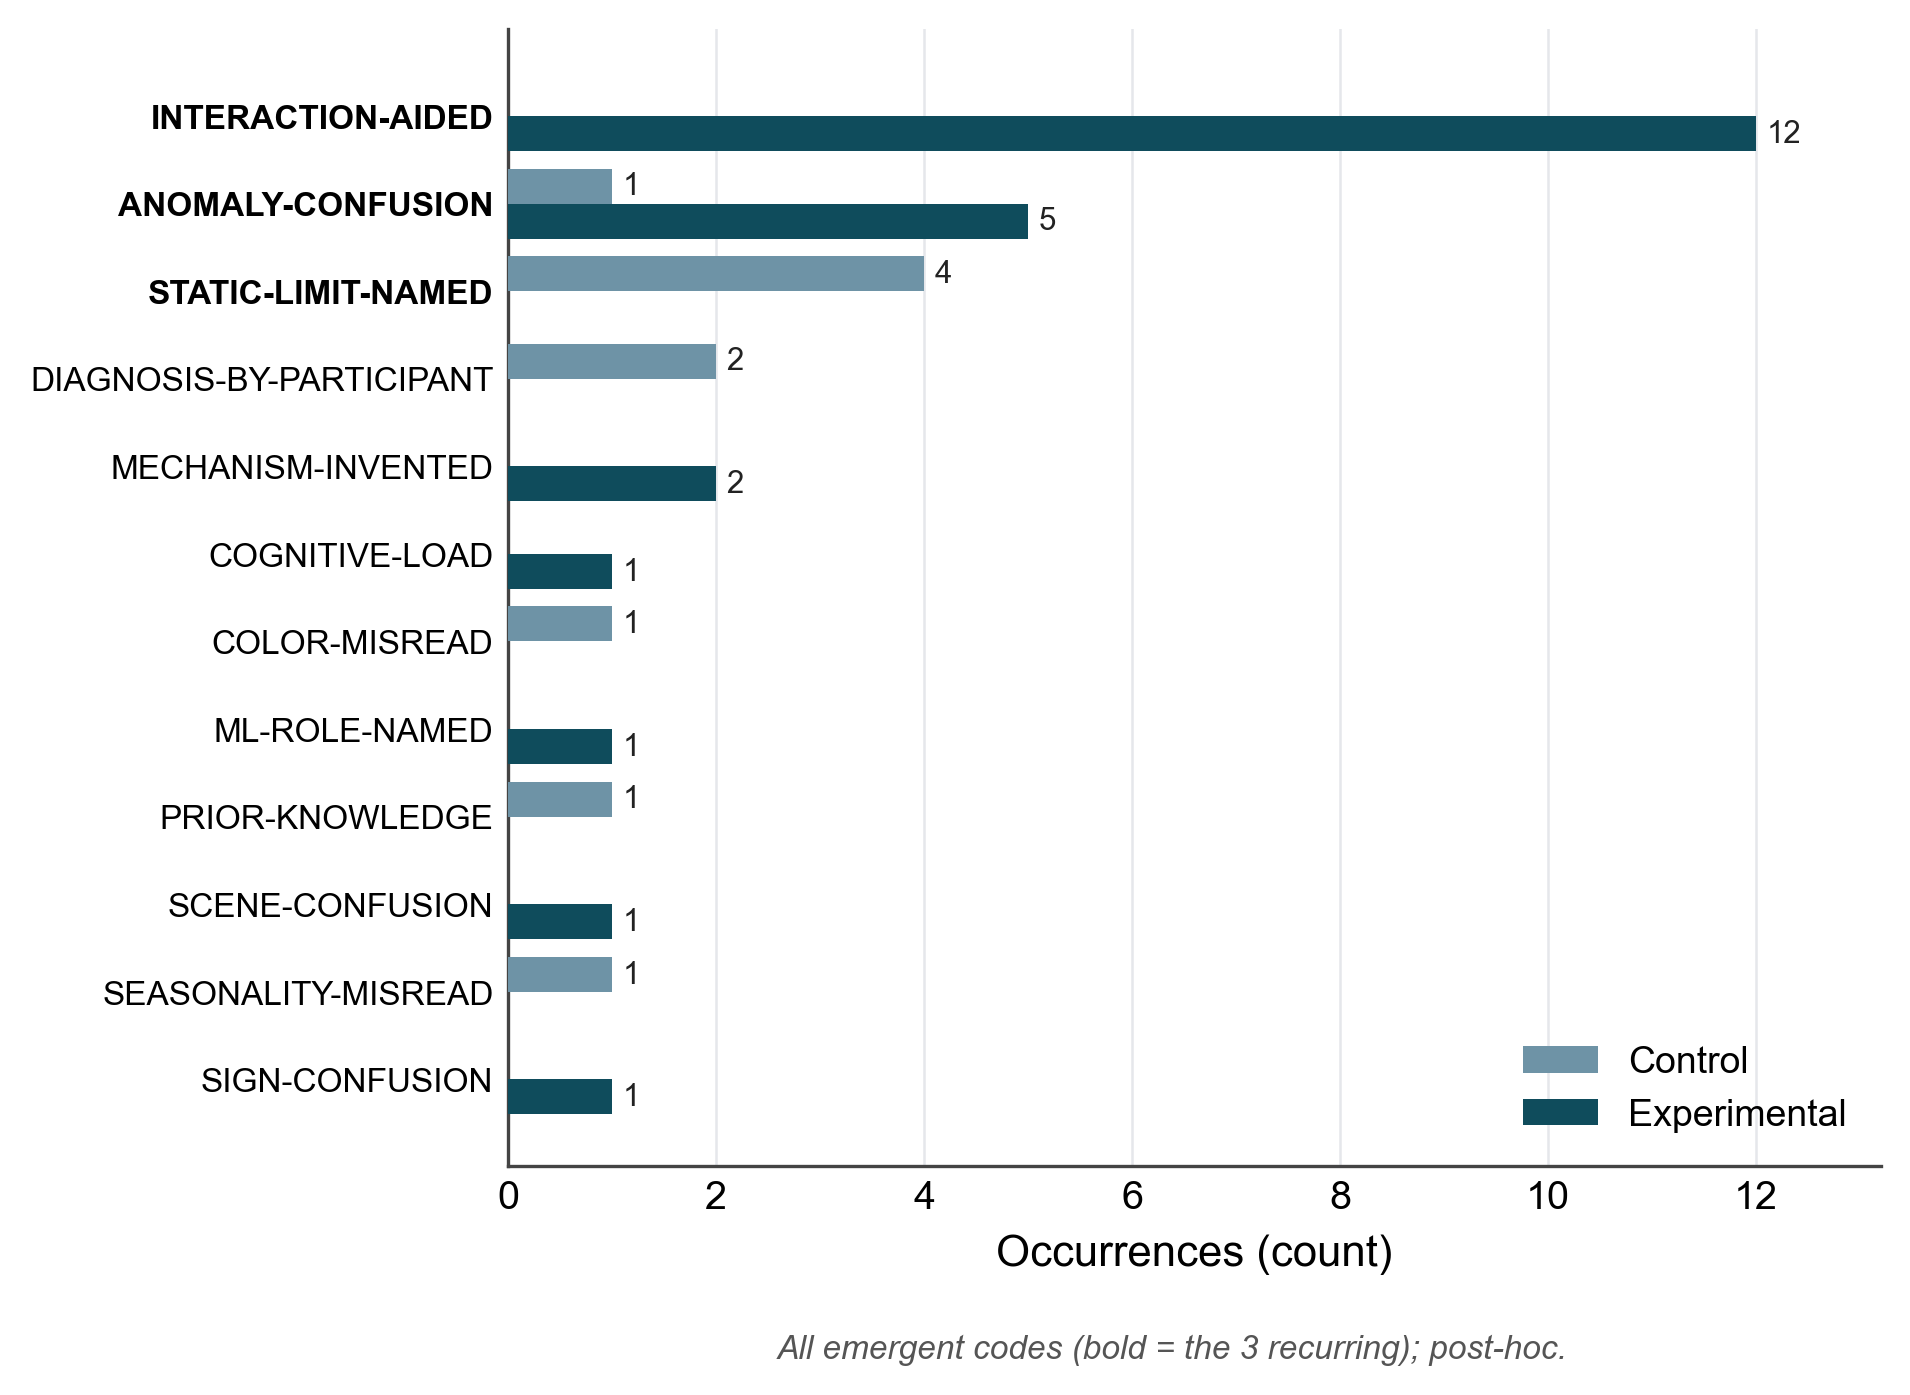
\includegraphics[width=\textwidth]{figures/results/S4_emergent_all_codes.png}
\caption[Tutti i codici emergenti per condizione]{L'elenco completo dei codici emergenti per condizione. Il grassetto segna i tre codici ricorrenti. Tutti sono post-hoc e non facevano parte della griglia definita a priori.}
\label{fig:emergent-full}
\end{figure}
